In diesem Kapitel werden die Rahmen- und Randbedienungen für das methodische Vorgehen der Evaluation großer Sprachmodelle für die Codegenerierung von webbasiertem Code festgehalten. Dies umfasst die Festlegung der verwendeten LLMs, die geprüfte Programmiersprachen, Framework zur Erstellung und Auswertung der Tests und Systeme für die Bereitstellung und Verarbeitung der Ergebnisse. Die Evaluierung der Modelle erfolgt in deutscher Sprache, was die Prompts und die Tests betrifft. Allein die Methodenbezeichnung ist in englischer Sprache.

\section{Definition der Evaluierungsziele}
%*   Dieser Abschnitt stellt sicher, dass die Evaluation messbar und reproduzierbar ist.

%*   Welche Aspekte der Codegenerierung sollen evaluiert werden? (z.B. Korrektheit des generierten Codes, Performance (Ausführungsgeschwindigkeit), Codequalität (Lesbarkeit, Wartbarkeit), Einhaltung von Coding Standards, Sicherheit, etc.)
Ausgehend von den in Kapitel \ref{sec:goals_of_the_work} gestellten Ziele dieser Arbeit, werden hier das Konzept und das Design für die Evaluation beschrieben. Wie werden die Ziele erreicht und welche Komponenten sind dazu erforderlich, um die Daten zu erheben und auszuwerten.\vspace{0.2cm}

Die Evaluation soll zeigen, ob die generierten Codes korrekt funktioniert und es nicht zu Laufzeitfehlern oder Deadlocks kommt. Des Weiteren wird evaluiert, ob der Code den gängigen Programmierstil entsprechen und welche Qualität der generierte Code ausweist. Hier liegt vor allen der Fokus auf Lesbarkeit und Einhaltung von Codingstandards. Als letzter Punkt soll die Dokumentation innerhalb des Codes geprüft werden. Je besser diese Ausfällt je leichter sind spätere Refactorings möglich.\vspace{0.2cm}

Was nicht im Fokus liegt und in den Test vernachlässigt wird, sind die Performance der Modelle und die Architekturen der Systeme auf denen die Modelle laufen. Es geht in erster Linie um den generierten Code und dessen Brauchbarkeit für die reelle Verwendung in der Praxis.\vspace{0.2cm}

%*   Welche konkreten Metriken werden zur Messung dieser Aspekte verwendet? (z.B. Anzahl der Fehler im generierten Code, Ausführungszeit in Millisekunden, statische Codeanalyse-Metriken, etc.)
Für die Messung der Fehler wird die \texttt{pass@k} Methode angewandt. Diese Methode baut auf einen mitgelieferten Test auf, der für jedes Problem vorhanden ist. Der Test, zusammen mit dem generierten Code ergeben einen ausführbaren testbaren Code. Jeder Test wird in einer Liste notiert und dazu das Ergebnis ob positiv oder negativ. Daraus kann dann mit der \texttt{pass@k} Methode die repräsentative Zuverlässigkeit des Modells für jedes Problem und anschließend für das gesamte Modell errechnet werden.\vspace{0.2cm}

Während die Evaluierung der Model mit dem Aufgaben des HumanEval-XL erfolgten, wird die Optimierung der Prompts an eigen erstellte Aufgaben erfolgen. Diese sind komplexer als die allgemeinen Aufgaben aus dem HumanEval-XL Benchmark. Hierbei soll untersucht werden, mit welchem Ansätzen Prompts im Bereich der Codegenerierung im Bereich der Webprogrammierung erfolgen kann. Der Aufbau der Aufgaben orientiert sich am HumanEval Benchmark. Es wird neben der Aufgabe auch ein Unittest vorgegeben. Somit kann der generierte Code mit Unittests geprüft werden. Um diese Test ausführen zu können, sind PHP Dateien erforderlich. Somit müssen die generierten Codes in Dateien gespeichert werden und können im Anschluss geprüft werden.

%Für die erweiterte Messung des PHP Codes kommt das Tool \texttt{phpmetrics} zum Einsatz. \texttt{phpmetrics} liefert eine Vielzahl an Metriken,mit der der Code analysiert werden kann. Bei diesem Tool liegt der Fokus auf die Ergebnisse von \texttt{Cyclomatic Complexity}, mit der die Komplexität des Codes gemessen wird. Auf den \texttt{Maintainability Index} zur Auswertung der Wartbarkeit. Diese ermittelt wie aufwändig es zukünftig ist den Code zu erweitern und bewertet die Lesbarkeit. Ein weiterer Parameter welcher hilft die Komplexität zu bewerten, ist der \texttt{Logical Lines of Code} Parameter. Ein weiteres Indiz zur Wartbar- und Lesbarkeit ist der \texttt{Method Length} Parameter. Ein weiterer Parameter zur Bewertung der Lesbarkeit ist der Parameter \texttt{Numbers of Parmeters}. Diese gibt die Anzahl der Parameter welche in die Methode übergeben werden. Eine hohe Anzahl kann ein Indiz dafür sein, das der Code schwerer zu lesen ist. Zur Bewertung der Dokumentation wird der Parameter \texttt{Comment Density} herangezogen.
%Mithilfe eines Python-Skripts wird der generierte Code mit \texttt{phpmetrics} evaluiert.\vspace{0.2cm}

%(SonarQube, wenn die Zeit es noch erlaubt)

%Mit dem SonarQube steht ein Auswertungstool zur Verfügung, welches neben qualitativen Codeanalyse noch eine Sicherheitsanalyse des Codes durchführt und die technischen Schulden ermittelt. Somit ist SonarQube eine Ergänzung zu \texttt{phpmetrics}. SonarQube wird eine lokale VM ausgeführt und mittels Integration werden die generierten Codes an den Server übermittelt.\vspace{0.2cm}

%Beide Verfahren \texttt{phpmetrics} und \texttt{SonarQube} benötigen für die Analyse Dateien. Somit müssen die Ergebnisse erst als Datei gespeichert werden, bevor die Tools mit der Analyse beginnen.

%---------------------------------------------------------------------------------------------------


\section{Auswahl der LLMs und deren Konfiguration}\label{subsec:llm_selection}
%*   Dieser Abschnitt legt die experimentelle Basis fest

%*   Welche LLMs werden konkret in den Experimenten verwendet? (Begründung basierend auf den Ergebnissen des Grundlagenkapitels)
Für die Evaluation werden experimentell einige freie und kommerzielle Modelle ausgewählt und miteinander verglichen. Hauptsächlich wurden bei den freien Modellen, jene ausgewählt welche den Fokus auf die Codegenerierung legen und mit diesem Argument beworben werden. Als Referenz soll das kommerzielle Modell \textit{Gemini 1.5} dienen, welches durch stetige Verbesserung und einer großen Nutzerzahl erstellt wurde.\vspace{0.2cm}

Im Folgenden werden die ausgewählten LLMs kurz vorgestellt und warum diese gewählt wurden. Die Reihenfolge stellt an dieser Stelle keine Wertung der LLM oder über deren generierten Inhalte dar.\vspace{0.2cm}

Das \textbf{Qwen2.5-Coder}-Modell zeichnet sich durch seine spezialisierte Architektur für die Codegenerierung aus. Trainiert, um sowohl syntaktisch korrekten als auch funktional hochwertigen Code zu produzieren, integriert es fortschrittliche Mechanismen zum Kontextverständnis und semantisch sinnvolle Ausgabe. Es findet Anwendung in verschiedenen Bereichen der Softwareentwicklung, insbesondere in der Web- und Anwendungsprogrammierung. Die Qwen2.5-Coder Modellbeschreibung ist \cite{qwen-2024} und \cite{hui-2024} entnommen und wird in den Arbeiten vertieft.\vspace{0.2cm}

\textbf{Deepseek-Coder-V2} ist die zweite Generation der Deepseek-Coder-Reihe und bietet verbesserte Fähigkeiten zur Codegenerierung und -optimierung. Das Modell nutzt fortschrittliche Suchalgorithmen, um präzisere und effizientere Codestücke zu erstellen. Es ist insbesondere für seine hohe Genauigkeit bei der Generierung komplexer Algorithmen und Datenstrukturen bekannt. Die Modellbeschreibung ist unter anderem aus \cite{deepseek-ai-2024} und \cite{cui-2024} entnommen. Des Weiteren wird in beiden Arbeiten das Modell mit verschiedenen Open-Source und Close-Source Modellen verglichen.\vspace{0.2cm} 

Die Modelle \textbf{Llama 3.1-Claude} und \textbf{Llama 3.1} gehören mit 8 Milliarden Parametern zu den kleineren Modellen von MetaAI. Beide Modelle basieren auf dem LLama3.1 Modell, das Llama3.1-Claude ist aber mit anderen Systemaufforderungen erstellt wurden. Hierfür wurden die Systemaufforderungen vom Claude Sonnet 3.5 der Firma Anthropic’s verwendet, nachzulesen unter \cite{ollama_page_llama31_claude}. Ein ähnliches Modell ist auf Hugging Face veröffentlicht \cite{huggingface_page_llama31_claude}. Eine Modelcard mit weiteren Informationen zum Modell, ist unter \cite{meta-llama-no-date} zu finden.\vspace{0.2cm}

\textbf{Mistral} ist ein modernes leistungsfähiges Sprachmodell, welches nicht speziell für die Codegenerierung und -analyse entwickelt wurde. Es verwendet fortschrittliche Transformer-Architekturen und ist für eine Vielzahl von Aufgaben einsetzbar. Darunter fallen beispielsweise natürliche Sprachverarbeitung, Textzusammenfassungen, maschinelle Übersetzung und Textklassifizierung. Dieses Modell ausgewählt, um ein Modell zu evaluieren, welches nicht speziell auf Codegenerierungsaufgaben trainiert wurde. In der Arbeit \cite{eberhardinger-2024} wurde Mistral, mit verschiedenen Modelle zur Spielecodegenerierung verglichen. Während in \cite{quan-2024} eine Evaluation für natürlichsprachlicher Erklärungen, Mistral mit anderen Modellen verglichen wurde.\vspace{0.2cm}

%\textbf{ChatGPT 3.5} und das Nachfolgemodell \textbf{ChatGPT 4}, entwickelt von OpenAI, sind vielseitig einsetzbare Close-Source Modelle. Neben allgemeinen textuellen Einsatzgebieten kann es für die Codegenerierung eingesetzt werden. Seit November 2022 ist das Modell ChatGPT 3.5 für alle kostenlos nutzbar und wird von sehr vielen Nutzer eingesetzt. Mit diesen Daten werden neue Modelle, wozu auch ChaGPT 4 zählt ständig neu trainiert. Dadurch werden die Modelle immer besser. Die Fallstudie \cite{ahmed-2025} die Bewertung des Nutzens von ChatGPT 4 für die Gestaltung einer barrierefreien Webseite. Eine Übersicht über die Modelle ist unter \cite{openai_model_overview} einsehbar.\vspace{0.2cm}

Mit \textbf{Gemini 1.5} präsentiert Google ein Modell zur Verarbeitung von natürlicher Sprache und stellt es zur freien Nutzung zur Verfügung. Genau wie ChatGPT nutzt auch Google die Nutzereingaben, um neue Modelle zu trainieren, was zur Weiterentwicklung für und somit zum neuen Modell \textbf{Gemini 2}. Wie in \cite{siam-2024} beschrieben, setzen auch die Gemini Modelle die Transformer-Architektur ein, was sie dazu befähigt, komplizierte Sprachmuster zu erkennen und präzise Vorhersagen zutreffen. In \cite{siam-2024} wird Gemini 1.5 mit Aufgaben zur Codegenerierung mit ChatGPT und Copilot vergleichen. Nach \cite{elgedawy-2024} kann sich das Gemini-Ultra-Modell beim MMLU-Benchmark sogar mit menschlichen Experten messen und erschließt eine breite Palette von Anwendungsbereichen. Hier wurden die Fähigkeiten zur Codegenerierung an Sicherheitsfragen im E-Commerce Bereich getestet. Ein Überblick über die Gemini Modelle ist unter \cite{google_gemini_model_overview} zu finden.\vspace{0.2cm}

Neben den genannten Quellen sind die Herstellerseite eine gute Quelle weiterführende Informationen einzuholen.\vspace{0.2cm}

Die Tabelle \ref{tab:selected_llms} zeigt zusammenfassend die ausgewählten Modelle.\vspace{0.2cm}

\begin{table}[!ht]
	\begin{tabular}{|l|l|l|c|c|c|c|}
		\hline
		\textbf{Modell} & \textbf{Param} & \textbf{Quantisierung} & \textbf{Größe} & \textbf{Sprache} & \textbf{offen} & \textbf{EXEC} \\
		\hline
		Qwen2.5-coder     & 32b &               q4\_K\_M &  19 GB &    DE & X & Ollama \\
		Deepseek-coder-V2 & 16b & lite-instruct-q5\_K\_S &  11 GB &    DE & X & Ollama \\
		Llama3.1-Claude   &  8b &                  q4\_0 & 4,7 GB &    DE & X & Ollama \\
		Llama3.1          &  8b &               q4\_K\_M & 4,7 GB & DE/EN & X & Ollama \\
		Llama3.2          &  3b &               q4\_K\_M & 2,0 GB & DE/EN & X & Ollama \\
		Llama3.3          & 70b &         instruct-q2\_K &  43 GB & DE/EN & X & Ollama \\
		Codellama         & 13b &                  q4\_0 & 7,4 GB &    DE & X & Ollama \\
		Mistral Small     & 22b &                  q4\_0 &  12 GB &    DE & X & Ollama \\
		Gemini 1.5 Pro    &k.A. &                   k.A. &   k.A. &    DE & - & online \\
		\hline
		\hline
	\end{tabular}
	\caption{Auswahl der LLMs für die Evaluierung}
	\label{tab:selected_llms}
\end{table}

%*   Welche spezifischen Parameter und Einstellungen der LLMs werden verwendet? (z.B. Temperatur, maximale Tokenanzahl, Top-p Sampling, etc.)
Die Einstellung für die Abfragen der Probleme wurden bei allen Modellen identisch gewählt.\vspace{0.2cm}

Für die Abfragen der Testprobleme wurde eine \textit{temperature} von $0.2$ gewählt. Ein niedriger Wert veranlasst die Modelle deterministischere und standardisierte Antworten zu geben und verhindert Kreativität und Zufälligkeit. Die Generierung von Programmcode soll konsistenten und präzisen Code liefern.\vspace{0.2cm}

Ein hoher \textit{top\_p} Wert verlangt von den Modellen eine Antwort die mit hoher Wahrscheinlichkeit richtig ist. Für die Codegenerierung sollten die wahrscheinlichsten und syntaktisch korrekten Token angewandt werden. Für die Abfragen wird hier ein Wert von $0.95$ angesetzt.\vspace{0.2cm}

Die maximale Anzahl Token sollte bei der Generierung von Code zwischen 20 und 1000 Token eingestellt werden, je nach Umfang der Antworten. Da hier nicht nur die Funktionsfähigkeit geprüft wird, sondern auch Struktur und Coding-Standards wird ein hoher Wert ausgewählt, sodass beispielsweise Kommentare ebenfalls enthalten sind können. Somit wird \textit{max\_token} auf sechshundert festgelegt.\vspace{0.2cm}

In der Tabelle \ref{tab:params_for_llms} sind die Werte in übersichtlicher kurzer Form noch einmal dargestellt.

\begin{table}[!ht]
	\begin{tabular}{|l|c|c|c|}
		\hline
		\textbf{Modell} & \textbf{Temp.} & \textbf{max. Token} & \textbf{Top-p} \\
		\hline
		Qwen2.5-coder     &  0.2 &       600 & 0.95 \\
		Deepseek-Coder-v2 &  0.2 &       600 & 0.95 \\
		Llama3.1          &  0.2 &  600/1200 & 0.95 \\
		Llama3.1-Claude   &  0.2 &       600 & 0.95 \\
		Llama3.2          &  0.2 &       600 & 0.95 \\
		Llama3.3          &  0.2 &       600 & 0.95 \\
		Mistral Small     &  0.2 &       600 & 0.95 \\
		Gemini 1.5 Pro    & k.A. &      k.A. & k.A. \\
		\hline
	\end{tabular}
	\centering
	\caption{Einstellungen der Modellparameter}
	\label{tab:params_for_llms}
\end{table}

Hinzu kommen weitere Parameter für die Modelle. Unter anderem wird der Parameter \textit{do\_sample} auf $False$ gesetzt, was die Modelle veranlasst den wahrscheinlichsten folgenden Token zu wählen und ein deterministisches Verhalten fördert. Ein weiterer Parameter ist \textit{return\_full\_text} der ebenfalls auf $False$ gesetzt wird. Dadurch werden nur die neu generierten Tokens zurückgegeben, was die Relevanz der Antworten fördert.\vspace{0.2cm}

%*   Werden die LLMs direkt über ihre APIs angesprochen oder werden Frameworks/Bibliotheken verwendet?
Alle Prompts welche die Probleme enthalten, werden mit Python Skripten abgefragt. Dies gilt für die offenen lokalen wie auch für die kommerziellen Modelle. Die Abfragen werden jeweils an die entsprechenden APIs abgesetzt. Als Frameworkfür die Abfragen der lokalen Modelle, kommt das Python \texttt{langchain} Framework zu Einsatz. Für die Modelle der Gemini-Reihe wird die Google eigene Bibliothek, \texttt{google.genai} verwendet. Dasselbe trifft für die Modelle von OpenAI zu. Hier kommt die Python Bibliothek \texttt{openai} zum Einsatz.

%---------------------------------------------------------------------------------------------------


\section{Design der Experimente}
%*   Dieser Abschnitt ist zentral für die Arbeit, da er die methodische Vorgehensweise der Evaluation beschreibt.
Das Experiment wird mit dem HumanEval-XL Benchmark durchgeführt. Dieser Benchmark besteht aus einer Reihe von 80 Tests in verschiedenen Programmiersprachen, die wie folgt aufgebaut sind,

\begin{myitemize}
	\item \textbf{task\_id}: Kennung der Datenprobe
	\item \textbf{prompt}: Anfrage für das Modell, Funktionsheader und Docstring
	\item \textbf{entry\_point}: Einstiegspunkt für den Test
	\item \textbf{test}: Test für die geforderte Funktion
	\item \textbf{description}: Beschreibung der Aufgabe
	\item \textbf{language}: Kennung der Programmiersprache
	\item \textbf{canonical\_solution}: Lösung für das Problem
	\item \textbf{natural\_language}: Ländersprache in der Datei
\end{myitemize}

Die Abbildung \ref{img:code_generation_humaneval} zeigt den Aufbau und damit alle wichtigen Bereiche des Benchmark-Tests.\vspace{0.2cm}

\begin{figure}[!ht]
	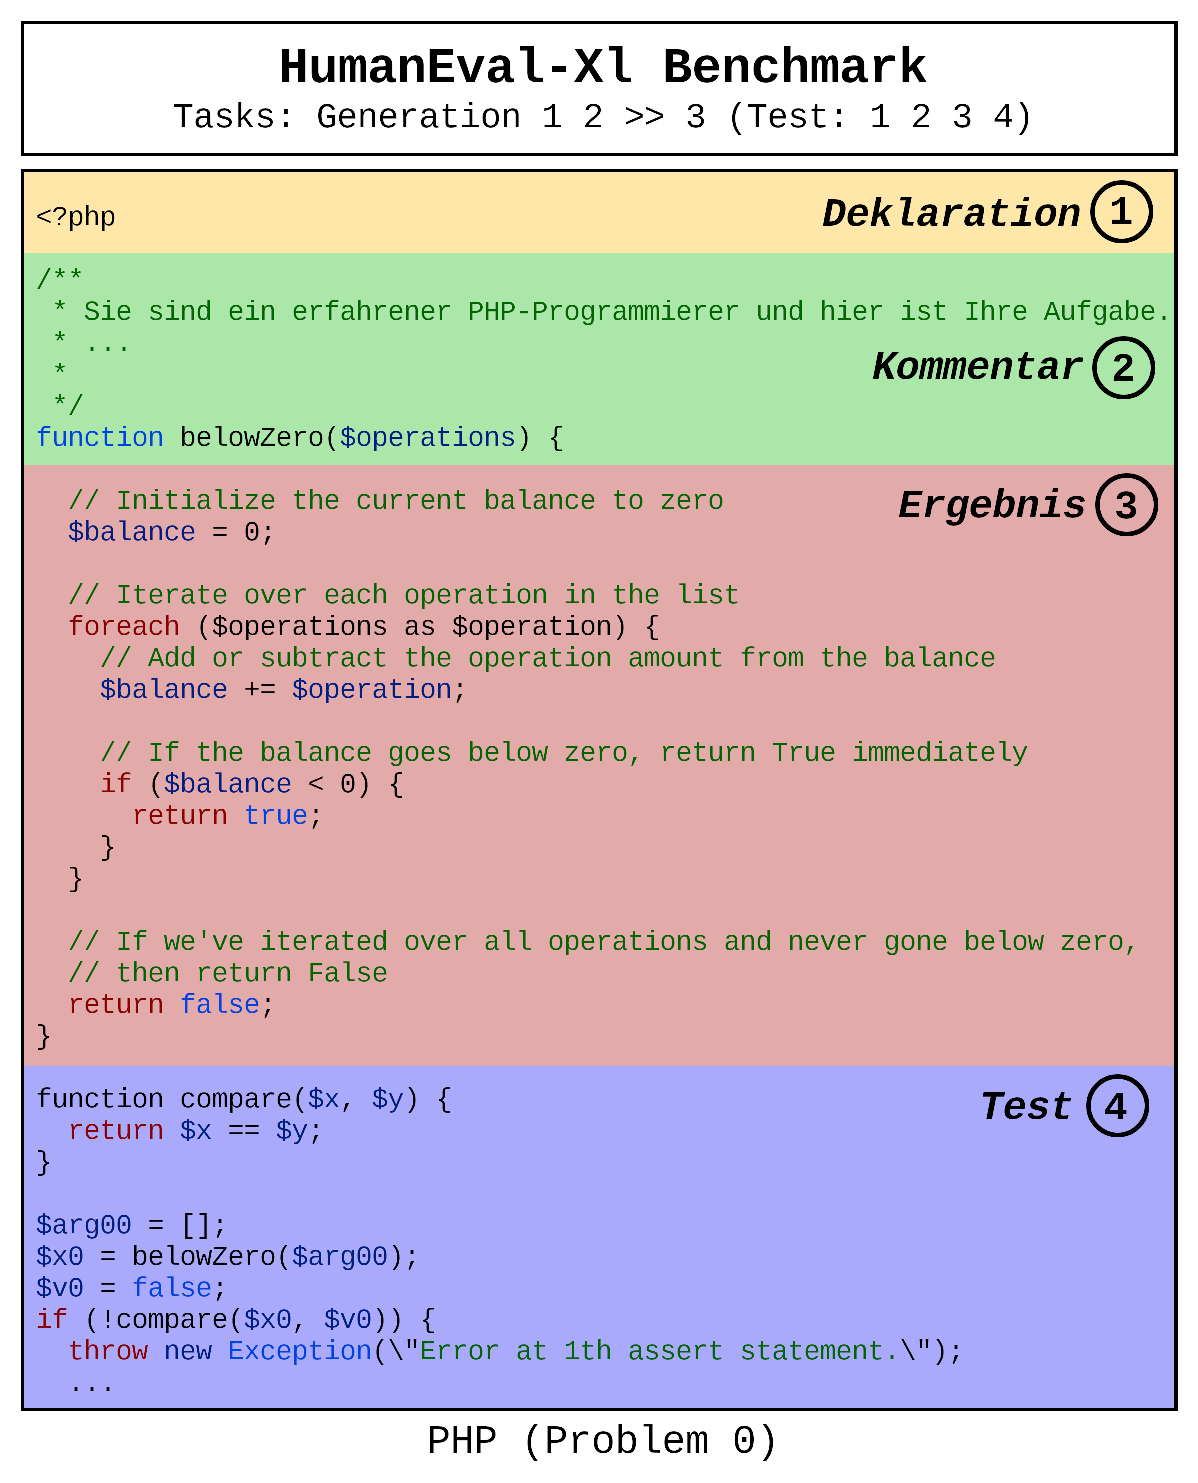
\includegraphics[width=0.8\textwidth]{content/chapter_intruduction/images/code_generation_humaneval_x.eps}
	\centering
	\caption{Codegeneration}
	\label{img:code_generation_humaneval}
\end{figure}

%*   Welche Arten von Code sollen generiert werden? (z.B. einfache HTML-Formulare, komplexe JavaScript-Funktionen, serverseitiger Code in Python/Node.js, etc.)
Um die Modelle zu evaluieren und ihre Fähigkeiten hinsichtlich der im Web vorherrschenden Programmiersprachen zu untersuchen, werden die Tests in den Programmiersprache(n) PHP (und JavaScript) vorgenommen. Dafür sollen die Modelle mehrfach einfache Funktionen generieren.\vspace{0.2cm}

%*   Wie werden die Testfälle für die Evaluation generiert? (z.B. manuelle Erstellung, automatische Generierung, Verwendung von bestehenden Code-Snippets, etc.) Wie groß ist der Umfang der Testfälle? (Anzahl der zu generierenden Code-Snippets)
Der Benchmark liefert die Tests mit. Dazu werden bereits in den Prompts die Namen der Methoden und die zu übergebenen Parameter angegeben, welche zu erstellen ist. Der jeweilige Test verwendet dann diesen Namen und übergibt die geforderten Parameter. Das Listing \ref{lst:example_prompt_test_by_humaneval_benchmark} zeigt ein Beispiel für einen mitgelieferten HumanEval-XL Test.

\begin{lstlisting}[language=php,caption={Beispiel für einen Test aus dem HumanEval-XL Benchmark},label=lst:example_prompt_test_by_humaneval_benchmark]
function compare($x, $y) {
	return $x == $y;
}
$arg00 = [3, 1, 2, 4, 5];
$x0 = median($arg00);
$v0 = 3;
if (!compare($x0, $v0)) {
	throw new Exception(\"Error at 1th assert statement.\");
}
\end{lstlisting}


%*   Wie werden die Ergebnisse der LLMs verglichen? (z.B. Vergleich mit Referenzcode, manuelle Überprüfung, automatische Tests, etc.)
Um die Modelle untereinander zu vergleichen, bekommen alle Modelle dieselben Prompts. Von jedem Prompt werden pro Modelle zehn Varianten erstellt. Die Ergebnisse werden in einer Liste chronologisch gespeichert. Diese Ergebnisse werden dann mittels der \texttt{pass@k} Metrik geprüft.

%---------------------------------------------------------------------------------------------------


\section{Konzeption des Prompt-Engineerings}
%*   Welche Strategien für das Prompt-Engineering werden untersucht? (z.B. Few-Shot-Prompting, Chain-of-Thought-Prompting, Verwendung von Code-Kommentaren als Prompts, etc.)
Die Prompts im HunamEval-XL Benchmark sind als Few-Shot-Prompts verfasst. Sie neben der eigentlichen Aufgabe sind noch Beispiel für die Eingabedaten und erwarteten Ergebnisse angegeben. Das Listing \ref{lst:example_prompt_by_humaneval_benchmark} zeigt ein Beispiel für einen Prompt.

\begin{lstlisting}[language=php,caption={Prompt Beispiel für  eine Aufgabe aus dem HumanEval-XL Benchmark},label=lst:example_prompt_by_humaneval_benchmark]
<?php

/**
* Sie sind ein erfahrener PHP-Programmierer und hier ist Ihre Aufgabe.
* Gib den Median der Elemente in der Liste l zurück.
* >>> median([3, 1, 2, 4, 5])
* 3
* >>> median([-10, 4, 6, 1000, 10, 20])
* 15.0
*
*/
function median($l){
\end{lstlisting}

%*   Wie werden die Prompts aufgebaut sein? (z.B. klare Anweisungen, Beispiele, Kontextinformationen, etc.)
Alle Prompts im Benchmark sind als Code-Kommentare aufgebaut. Als letzte Zeile ist der Methodenname angegeben. Somit soll sichergestellt werden, dass die erstellten Tests funktionieren.\vspace{0.2cm}

%*   Werden verschiedene Prompt-Varianten für die gleichen Code-Generierungsaufgaben verwendet, um deren Einfluss auf die Ergebnisse zu untersuchen?


%*   Dieser Abschnitt ist besonders wichtig, da er sich mit der Optimierung der LLMs durch Prompt-Engineering beschäftigt.

%---------------------------------------------------------------------------------------------------


\section{Evaluationsumgebung}
%*   Welche Hardware und Software werden für die Experimente verwendet? (z.B. CPU, GPU, Betriebssystem, Programmiersprachen, Bibliotheken, etc.)
Die freien Modelle laufen auf einem Debian 12 System, welches mit 16 CPUs und 32 GB RAM ausgestattet ist. Um zusätzlichen Speicher zu erhalten, wurde eine 100 GB Swap Partition genutzt. Für die Bereitstelle ist das freie Framework Ollama zum Einsatz gekommen.\vspace{0.2cm}

Die Hardware Auf die kommerziellen Modelle kann kein Einfluss auf die Systeme genommen werden.\vspace{0.2cm}

Alle erstellten Codes und Ergebnisse werden dokumentiert und im Anhang eingefügt, sodass einen die Evaluierungen nachvollzogen werden können. Des Weiteren werden alle Daten und Dateien unter \href{https://github.com/willi-pahl/master-thesis}{https://github.com/willi-pahl/master-thesis} bereitgestellt.\vspace{0.2cm}

%*   Wie wird die Reproduzierbarkeit der Experimente sichergestellt? (z.B. Verwendung von Versionskontrolle, Dokumentation der Umgebung, etc.)

\begin{tcolorbox}[
	enhanced,
	colback=red!5!white,
	colframe=red!75!black!50,
	title= Mein roter Faden
	]
	Hier kommen noch Optimierungsangaben, die stehen zurzeit nicht fest.
\end{tcolorbox}
